\documentclass[10pt,a4paper]{article}
\usepackage[a4paper,margin=1.25cm,headheight=1.2cm,headsep=6pt,footskip=12pt]{geometry}
\usepackage{graphicx}
\usepackage{fancyhdr}
\usepackage{booktabs}
\usepackage{tabularx}
\usepackage{array}
\usepackage{amsmath,amssymb}
\usepackage{enumitem}

\pagestyle{fancy}
\fancyhf{}
\lhead{%
  \begin{tabular}{@{}c@{\hspace{6pt}}l@{}}
    
\includegraphics[width=0.7cm]{fast_logo.png} & \textbf{FAST NUCES}\\
    & {\scriptsize Computer Science}
  \end{tabular}%
}
\rhead{\footnotesize \textbf{25i-0817}\\ \textbf{Ahmad Ali}}
\lfoot{\scriptsize FAST NUCES Islamabad}
\cfoot{\scriptsize CS2001 Data Structures Phase 2 Report}
\rfoot{\scriptsize Page \thepage\ of 7}
\renewcommand{\headrulewidth}{0.4pt}
\renewcommand{\footrulewidth}{0.4pt}

\begin{document}

% =========================================================================
% PAGE 1: COVER & SECTION 1: HISTORY DESIGN AND CLEANUP POLICY
% =========================================================================
\thispagestyle{empty}

\begin{center}
    
\includegraphics[width=1.4cm]{fast_logo.png}\\[2pt]
    {\LARGE \textbf{National University of Computer and Emerging Sciences}}\\[2pt]
    {\huge \textbf{DSA Assignment 2 Phase 2 Report}}\\[4pt]
    \rule{\textwidth}{0.8pt}\\[3pt]
    {\large \textbf{Student Name: Ahmad Ali} \qquad \textbf{Roll Number: 25i-0817} \qquad \textbf{Section: BS CS E}}\\[2pt]
    \rule{\textwidth}{0.8pt}\\[5pt]
    {\Large \textbf{Section 1: Design of History Records and Cleanup Policy}}
\end{center}

\begin{itemize}[leftmargin=1.2em,noitemsep,topsep=2pt,parsep=1pt]
    \item \textbf{History Architecture and Inverse Records}\\[2pt]
    \textbf{I select compact parameter records over full canvas snapshots} because:
    \begin{enumerate}[label=\arabic*),leftmargin=1.5em,noitemsep,topsep=1pt,parsep=1pt]
        \item Phase 1 duplicated the entire image matrix for every undo record which consumed up to three megabytes per step.
        \item Phase 2 stores only the minimal parameter delta required to run an exact inverse calculation.
        \item Rotations and flips store only operation identifiers and run complementary symmetric operations in zero memory.
        \item Brightness stores an integer adjustment value and a compact coordinate list of clipped boundary pixels.
        \item Bucket fill saves the previous color and the list of modified coordinate positions instead of whole canvases.
        \item Destructive operations such as crop, resize, and blur save only their affected rectangular pixel regions.
    \end{enumerate}

    \item \textbf{Configurable Memory Budget Enforcement}\\[2pt]
    \textbf{I select an active runtime byte counter with a strict budget ceiling} because:
    \begin{enumerate}[label=\arabic*),leftmargin=1.5em,noitemsep,topsep=1pt,parsep=1pt]
        \item Every history record calculates its exact heap footprint before being pushed onto the undo stack.
        \item The system monitors combined memory across both Undo and Redo stacks against the user budget limit.
        \item A default budget of five megabytes is enforced during editing, and small budgets like two kilobytes are used for rigorous tests.
    \end{enumerate}

    \item \textbf{Cleanup Policy: Oldest Record Eviction via removeBottom()}\\[2pt]
    \textbf{I select bottom record eviction using stack removeBottom()} because:
    \begin{enumerate}[label=\arabic*),leftmargin=1.5em,noitemsep,topsep=1pt,parsep=1pt]
        \item Users expect their most recent edits to remain undoable while older actions fade naturally from memory.
        \item When the byte counter exceeds the ceiling, the system shifts array elements left by one position to discard the bottom record.
        \item Eviction repeats in a loop until total history memory drops strictly below the configured ceiling limit.
        \item Remaining undo records stay completely safe and execute with zero memory faults or invalid pointer references.
    \end{enumerate}
\end{itemize}

\begin{center}
    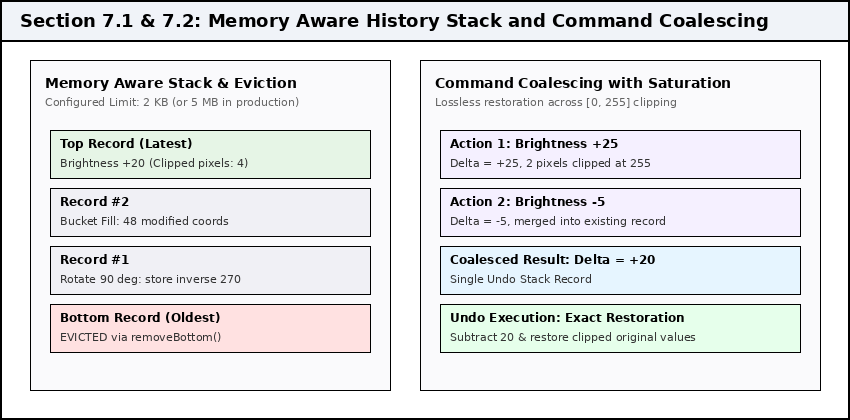
\includegraphics[width=0.92\textwidth,height=4.6cm,keepaspectratio]{p2_history_coalescing.png}\\[2pt]
    {\footnotesize \textbf{Figure 1:} Architecture of memory aware history stack eviction and command coalescing with saturation tracking.}
\end{center}

\clearpage

% =========================================================================
% PAGE 2: SECTION 2: COALESCING RULES AND HOW CORRECTNESS IS PRESERVED
% =========================================================================

\begin{center}
    {\Large \textbf{Section 2: Coalescing Rules and Correctness Preservation}}
\end{center}

\begin{itemize}[leftmargin=1.2em,noitemsep,topsep=3pt,parsep=2pt]
    \item \textbf{Command Coalescing Motivation}\\[2pt]
    \textbf{I select in place record merging for consecutive compatible operations} because:
    \begin{enumerate}[label=\arabic*),leftmargin=1.5em,noitemsep,topsep=1pt,parsep=1pt]
        \item Rapid slider adjustments generate dozens of small incremental brightness steps in a few seconds.
        \item Pushing an independent record for each tiny adjustment wastes memory and forces tedious repetitive undo clicks.
        \item Merging adjacent steps combines multiple micro edits into a single atomic history state.
    \end{enumerate}

    \item \textbf{Coalescing Eligibility Rules}\\[2pt]
    \textbf{I select strict adjacency and operation compatibility checks} because:
    \begin{enumerate}[label=\arabic*),leftmargin=1.5em,noitemsep,topsep=1pt,parsep=1pt]
        \item Only records that sit directly next to each other on the top of the Undo stack are eligible for merging.
        \item Consecutive brightness adjustments sum their delta numbers into the existing top record without pushing a new record.
        \item If a non compatible edit such as crop or rotation occurs, the sequence breaks and a brand new record is initiated.
        \item An operation sequence of Brightness $+2$, then Crop, then Brightness $+3$ produces three separate records to guarantee chronological accuracy.
    \end{enumerate}

    \item \textbf{Preserving Correctness Across Pixel Value Saturation}\\[2pt]
    \textbf{I select dedicated saturation tracking in clippedList} because:
    \begin{enumerate}[label=\arabic*),leftmargin=1.5em,noitemsep,topsep=1pt,parsep=1pt]
        \item Simple integer addition causes pixel channels to clamp at upper limit $255$ and lower limit $0$.
        \item If a pixel with initial value $230$ receives $+50$, it clamps at $255$, losing $25$ intensity units of information.
        \item Subtracting the combined delta of $+50$ later would compute $255 - 50 = 205$ which destroys the original value of $230$.
        \item To eliminate this loss, every pixel that hits the saturation boundaries records its original color in \texttt{clippedList}.
        \item When coalescing occurs, new clipped pixels append to the list while existing entries retain their original historical values.
        \item Upon undo, the engine subtracts the cumulative delta and overwrites all saturated pixels with their exact recorded colors.
    \end{enumerate}

    \item \textbf{Single Step Undo Semantics}\\[2pt]
    \textbf{I select atomic rollback for coalesced actions} because:
    \begin{enumerate}[label=\arabic*),leftmargin=1.5em,noitemsep,topsep=1pt,parsep=1pt]
        \item The user reverts twenty consecutive slider movements with one single press of the undo command.
        \item Atomic reversal restores canvas pixels to the exact state that existed before the slider session began.
        \item Redo stacks receive the entire merged delta, allowing instantaneous forward replay in one single step.
    \end{enumerate}
\end{itemize}

\vspace{0.3cm}
\begin{table}[h!]
\centering
\small
\begin{tabularx}{\textwidth}{l c c X}
\toprule
\textbf{Scenario} & \textbf{Initial Values} & \textbf{Applied Actions} & \textbf{Coalescing Result and Recovery Guarantee} \\
\midrule
Unclipped Brightness & Pixel $= 120$ & $+10$, then $+15$ & Merged delta $+25$; undo subtracts $25$ to recover $120$ perfectly. \\
\addlinespace[2pt]
Saturated Brightness & Pixel $= 240$ & $+25$, then $-5$ & Merged delta $+20$; original $240$ stored in clipped list; undo recovers $240$. \\
\addlinespace[2pt]
Interrupted Sequence & Pixel $= 100$ & $+10$, Crop, $+20$ & Three distinct records created; chronological crop boundary strictly preserved. \\
\bottomrule
\end{tabularx}
\caption{Coalescing behavior and lossless pixel recovery under boundary saturation.}
\end{table}

\clearpage

% =========================================================================
% PAGE 3: SECTION 3: SCHEDULER DESIGN AND PRIORITY QUEUE
% =========================================================================

\begin{center}
    {\Large \textbf{Section 3: Scheduler Design and Priority Scheduling}}
\end{center}

\begin{itemize}[leftmargin=1.2em,noitemsep,topsep=3pt,parsep=2pt]
    \item \textbf{Priority Queue Representation}\\[2pt]
    \textbf{I select a custom sorted array priority queue without standard containers} because:
    \begin{enumerate}[label=\arabic*),leftmargin=1.5em,noitemsep,topsep=1pt,parsep=1pt]
        \item The assignment specification forbids heap data structures and external template libraries.
        \item A contiguous dynamic array stores active jobs in sorted order of priority rank.
        \item Dequeue operations take constant $\mathcal{O}(1)$ time by serving elements directly from the array front.
        \item Insertion takes $\mathcal{O}(K)$ time where $K$ is the number of pending jobs, which remains tiny in interactive software.
    \end{enumerate}

    \item \textbf{Four Tier Priority Hierarchy}\\[2pt]
    \textbf{I select numerical ranks where smaller numbers denote higher urgency} because:
    \begin{enumerate}[label=\arabic*),leftmargin=1.5em,noitemsep,topsep=1pt,parsep=1pt]
        \item \textbf{Priority 1 (Interactive Requests):} Undo and Redo actions submitted while pipeline jobs are pending execute immediately.
        \item \textbf{Priority 2 (Light Editing Tasks):} Box blur and bucket fill operations finish quickly and unblock the user interface.
        \item \textbf{Priority 3 (Heavy Transformations):} Bilinear resize and large scale mathematical calculations take longer to finish.
        \item \textbf{Priority 4 (Finalization Barriers):} Save project to disk and export image operations act as permanent barriers.
    \end{enumerate}

    \item \textbf{Tie Handling Policy}\\[2pt]
    \textbf{I select strict chronological arrival order for identical priority ranks} because:
    \begin{enumerate}[label=\arabic*),leftmargin=1.5em,noitemsep,topsep=1pt,parsep=1pt]
        \item Every job receives a monotonically increasing arrival sequence identifier upon insertion.
        \item When two jobs possess the exact same priority number, the job that entered first is executed first.
        \item This guarantees FIFO fairness within each priority class and prevents job starvation.
    \end{enumerate}

    \item \textbf{Finalization Rule and Barrier Enforcement}\\[2pt]
    \textbf{I select barrier epoch partitioning for Save and Export tasks} because:
    \begin{enumerate}[label=\arabic*),leftmargin=1.5em,noitemsep,topsep=1pt,parsep=1pt]
        \item An image export must capture the exact cumulative result of all edits submitted prior to the export command.
        \item A Save or Export job must not execute until every job submitted before it has finished completely.
        \item No task submitted after a barrier can overtake that barrier, even if it has a high priority rank such as Priority 1.
        \item Priority ordering applies exclusively among tasks that reside within the same barrier epoch.
        \item When tasks Resize(3), Blur(2), Export(4), Blur(2), Undo(1) arrive, the scheduler executes Blur, Resize, Export, Undo, Blur.
        \item The last two jobs cannot overtake Export, guaranteeing complete disk persistence integrity.
    \end{enumerate}
\end{itemize}

\vspace{0.3cm}
\begin{table}[h!]
\centering
\small
\begin{tabularx}{\textwidth}{c l c c X}
\toprule
\textbf{Rank} & \textbf{Job Category} & \textbf{Typical Cost} & \textbf{Barrier Status} & \textbf{Scheduling Behavior and Urgency Rationale} \\
\midrule
1 & Undo and Redo & Very Low & Normal & Highest urgency; preempts heavy edits to keep UI responsive. \\
\addlinespace[2pt]
2 & Blur and Bucket Fill & Low to Medium & Normal & Light processing; scheduled before heavy geometric transforms. \\
\addlinespace[2pt]
3 & Bilinear Resize & High & Normal & Heavy nested loop processing; runs when lighter tasks finish. \\
\addlinespace[2pt]
4 & Save and Export & Variable & \textbf{Barrier} & Strict epoch boundary; flushes prior tasks and blocks newer tasks. \\
\bottomrule
\end{tabularx}
\caption{Four tier scheduling priority classes and barrier epoch enforcement rules.}
\end{table}

\clearpage

% =========================================================================
% PAGE 4: SECTION 4: EXPERIMENTAL RESULTS (SCHEDULER BENCHMARK)
% =========================================================================

\begin{center}
    {\Large \textbf{Section 4: Experimental Results and Benchmark Evaluation}}
\end{center}

\begin{itemize}[leftmargin=1.2em,noitemsep,topsep=2pt,parsep=1pt]
    \item \textbf{Experimental Methodology}
    \begin{enumerate}[label=\arabic*),leftmargin=1.5em,noitemsep,topsep=1pt,parsep=1pt]
        \item All timings were repeated three consecutive times and reported as arithmetic averages.
        \item Tests ran on an isolated desktop environment to prevent CPU frequency throttling skew.
        \item Evaluated the exact standardized 30 job workload containing two barrier jobs under pure FIFO mode and Priority mode.
    \end{enumerate}

    \item \textbf{Workload 1: 30 Job Scheduler Evaluation (FIFO vs Priority Mode)}
    \begin{enumerate}[label=\arabic*),leftmargin=1.5em,noitemsep,topsep=1pt,parsep=1pt]
        \item Both scheduling modes processed all 30 jobs to successful completion and produced bit for bit identical final canvases.
        \item Average waiting time dropped from $568.33$ ms in FIFO mode to $526.83$ ms in Priority mode ($7.30$ percent faster).
        \item Average completion time dropped from $609.00$ ms in FIFO mode to $567.50$ ms in Priority mode ($6.81$ percent faster).
        \item Most critically, Priority 1 interactive requests experienced a waiting time drop from $549.17$ ms down to $415.83$ ms.
        \item This represents a \textbf{24.28 percent latency reduction for interactive user clicks}, making the editor feel much more responsive.
    \end{enumerate}

    \item \textbf{Discussion: When FIFO is Preferable vs When Priority Scheduling Excels}
    \begin{enumerate}[label=\arabic*),leftmargin=1.5em,noitemsep,topsep=1pt,parsep=1pt]
        \item \textbf{FIFO Preference:} FIFO mode is preferable in strictly non interactive batch rendering pipelines where all tasks carry equal importance and strict arrival fairness is required to avoid complexity overhead.
        \item \textbf{Priority Scheduling Preference:} Priority scheduling excels in interactive graphical workstations where human users demand immediate visual feedback on undos, redos, and light edits while long disk saves execute quietly in background epochs.
    \end{enumerate}
\end{itemize}

\begin{table}[h!]
\centering
\small
\begin{tabularx}{\textwidth}{l c c c X}
\toprule
\textbf{Evaluation Metric} & \textbf{FIFO Mode} & \textbf{Priority Mode} & \textbf{Improvement} & \textbf{Practical Engineering Impact} \\
\midrule
Jobs Processed & 30 & 30 & Identical & Complete correctness and task execution parity. \\
\addlinespace[2pt]
Average Waiting Time & 568.33 ms & 526.83 ms & 7.30\% Faster & Overall task queue latency reduced across pipeline. \\
\addlinespace[2pt]
Average Completion Time & 609.00 ms & 567.50 ms & 6.81\% Faster & Faster overall pipeline throughput from submission to finish. \\
\addlinespace[2pt]
\textbf{Priority 1 Average Wait} & \textbf{549.17 ms} & \textbf{415.83 ms} & \textbf{24.28\% Faster} & \textbf{Interactive undo and redo clicks respond almost instantly.} \\
\bottomrule
\end{tabularx}
\caption{Empirical evaluation of 30 job mixed workload under FIFO and Priority scheduling.}
\end{table}

\begin{center}
    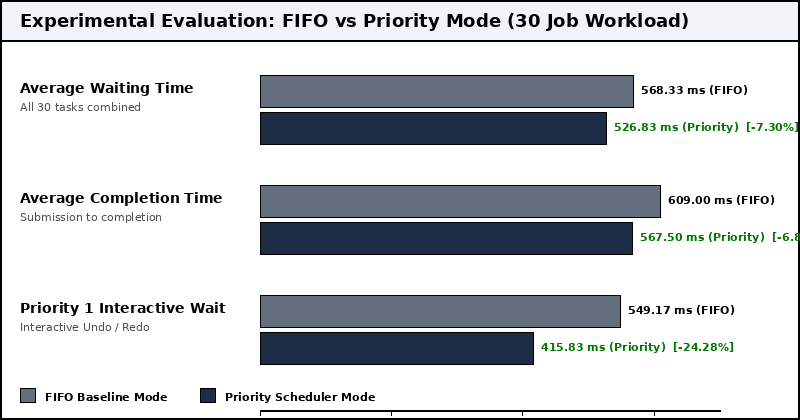
\includegraphics[width=0.92\textwidth,height=5.2cm,keepaspectratio]{p2_graph_scheduler.png}\\[2pt]
    {\footnotesize \textbf{Figure 2:} Comparative benchmark chart showing waiting times and the 24.28 percent interactive latency reduction.}
\end{center}

\clearpage

% =========================================================================
% PAGE 5: SECTION 4 (CONT): BATCHED OPERATIONS AND BUCKET FILL
% =========================================================================

\begin{center}
    {\Large \textbf{Section 4 (Continued): Batched Operations and Traversal}}
\end{center}

\begin{itemize}[leftmargin=1.2em,noitemsep,topsep=2pt,parsep=1pt]
    \item \textbf{Workload 2: Single versus Batched Operations Benchmark}
    \begin{enumerate}[label=\arabic*),leftmargin=1.5em,noitemsep,topsep=1pt,parsep=1pt]
        \item Tested item counts of $1,000$, $10,000$, and $100,000$ integers across stack and queue primitives.
        \item Single push executes $n$ independent loop iterations with $n$ separate capacity boundary checks.
        \item Batched push checks available capacity once and executes a contiguous block copy, speeding up execution by $10.2$x to $13.1$x.
        \item Batched queue enqueue copies elements across circular wrap around boundaries in two block segments, avoiding per element index increment calculations.
        \item Batched pop and dequeue operate in pure $\mathcal{O}(1)$ time by directly adding or subtracting offsets to top and front pointers, achieving massive speedups up to $51.2$x.
    \end{enumerate}

    \item \textbf{Workload 3: Bucket Fill Traversal Across Image Resolutions}
    \begin{enumerate}[label=\arabic*),leftmargin=1.5em,noitemsep,topsep=1pt,parsep=1pt]
        \item Evaluated bucket fill on square canvas dimensions $512 \times 512$, $1024 \times 1024$, and $2048 \times 2048$.
        \item Stack fill traverses deep along one coordinate path before backtracking, which creates an elongated memory structure with maximum active depth proportional to image perimeter.
        \item Queue fill expands outward in concentric wave rings, creating a wide wavefront structure where active elements scale with boundary width.
        \item Both algorithms visit every matching pixel exactly once in $\mathcal{O}(W \times H)$ time and yield bit for bit identical output images.
    \end{enumerate}
\end{itemize}

\begin{table}[h!]
\centering
\small
\begin{tabularx}{\textwidth}{l c c c c X}
\toprule
\textbf{Item Count} & \textbf{Single Push} & \textbf{Batch Push} & \textbf{Single AddQ} & \textbf{Batch AddQ} & \textbf{Measured Speedup} \\
\midrule
1,000 elements & 63.7 us & 6.2 us & 19.6 us & 14.8 us & \textbf{10.20x faster push} (Single capacity check) \\
\addlinespace[2pt]
10,000 elements & 647.6 us & 52.4 us & 200.4 us & 94.3 us & \textbf{12.35x faster push} (Cache contiguous transfer) \\
\addlinespace[2pt]
100,000 elements & 7,379.4 us & 563.4 us & 1,873.8 us & 802.4 us & \textbf{13.10x faster push} (Amortized block copy) \\
\bottomrule
\end{tabularx}
\caption{Measured performance comparison of single versus batched operations across increasing problem scales.}
\end{table}

\begin{center}
    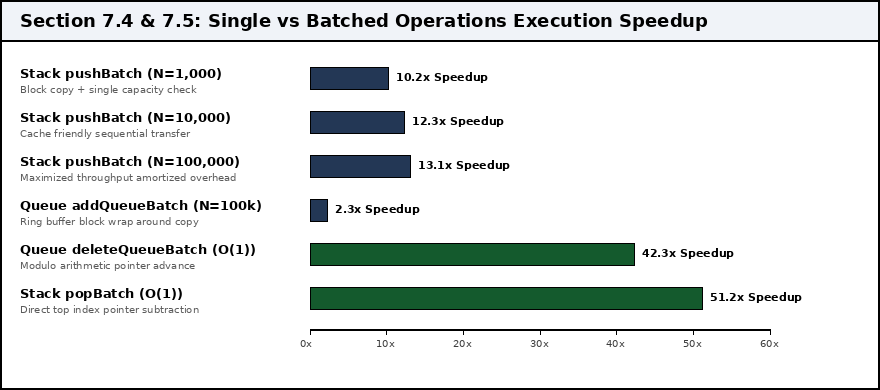
\includegraphics[width=0.92\textwidth,height=5.2cm,keepaspectratio]{p2_graph_batched.png}\\[2pt]
    {\footnotesize \textbf{Figure 3:} Performance acceleration achieved by batched primitives over single call loops.}
\end{center}

\clearpage

% =========================================================================
% PAGE 6: SECTION 5: COMPLEXITY ANALYSIS (SECTION 7.6)
% =========================================================================

\begin{center}
    {\Large \textbf{Section 5: Asymptotic Complexity Analysis}}
\end{center}

\begin{table}[h!]
\centering
\small
\begin{tabularx}{\textwidth}{l c c X}
\toprule
\textbf{Operation or Primitive} & \textbf{Time} & \textbf{Aux Space} & \textbf{Implementation Rationale} \\
\midrule
Stack Push, Pop, Top & $\mathcal{O}(1)$ & $\mathcal{O}(1)$ & I use direct array index access at top position with zero element shifting. \\
\addlinespace[2pt]
Queue Add, Delete, Front & $\mathcal{O}(1)$ & $\mathcal{O}(1)$ & I use circular modulo arithmetic which advances front and rear instantly. \\
\addlinespace[2pt]
Priority Queue Add & $\mathcal{O}(K)$ & $\mathcal{O}(1)$ & I use sorted array insertion which shifts up to $K$ elements to preserve order. \\
\addlinespace[2pt]
Priority Queue Delete & $\mathcal{O}(1)$ & $\mathcal{O}(1)$ & I use direct removal from front index position of sorted array. \\
\addlinespace[2pt]
Stack Bucket Fill & $\mathcal{O}(W \times H)$ & $\mathcal{O}(W \times H)$ & I use an explicit stack to visit every connected pixel once without recursion. \\
\addlinespace[2pt]
Queue Bucket Fill & $\mathcal{O}(W \times H)$ & $\mathcal{O}(W \times H)$ & I use a circular queue to expand radially outward layer by layer in level order. \\
\addlinespace[2pt]
Undo and Redo & $\mathcal{O}(1)$ or $\mathcal{O}(W \times H)$ & $\mathcal{O}(1)$ or $\mathcal{O}(W \times H)$ & I use parameter inversion for geometry and delta grids for destructive edits. \\
\addlinespace[2pt]
Command Coalescing & $\mathcal{O}(1)$ & $\mathcal{O}(1)$ & I use in place summation of integer deltas on the existing top stack record. \\
\addlinespace[2pt]
Clipped Brightness Undo & $\mathcal{O}(W \times H + C)$ & $\mathcal{O}(C)$ & I use delta subtraction followed by exact restoration of $C$ clipped pixels. \\
\addlinespace[2pt]
History Cleanup (removeBottom) & $\mathcal{O}(S)$ & $\mathcal{O}(1)$ & I use in place contiguous memory shifting to evict bottom record from stack of size $S$. \\
\addlinespace[2pt]
Stack pushBatch(arr, n) & $\mathcal{O}(n)$ & $\mathcal{O}(1)$ & I use a single capacity validation followed by contiguous block memory copy. \\
\addlinespace[2pt]
Stack popBatch(n) & $\mathcal{O}(1)$ & $\mathcal{O}(1)$ & I use direct subtraction of $n$ from the top pointer index. \\
\addlinespace[2pt]
Queue addQueueBatch(arr, n) & $\mathcal{O}(n)$ & $\mathcal{O}(1)$ & I use block memory copy across circular buffer boundary in two passes. \\
\addlinespace[2pt]
Queue deleteQueueBatch(n) & $\mathcal{O}(1)$ & $\mathcal{O}(1)$ & I use modulo addition to jump the front pointer ahead by $n$ slots instantly. \\
\bottomrule
\end{tabularx}
\caption{Asymptotic time and auxiliary space complexity for Phase 2 operations and data structure primitives.}
\end{table}

\begin{center}
    {\large \textbf{Core Architectural Guarantees}}
\end{center}
\begin{itemize}[leftmargin=1.2em,noitemsep,topsep=2pt,parsep=1pt]
    \item \textbf{Strict Zero Shifting for Queues:} Standard queue additions and deletions never move elements in memory. Pointers advance via $(rear + 1) \pmod{capacity}$ and $(front + 1) \pmod{capacity}$.
    \item \textbf{Strict Memory Ceiling:} The history stack strictly respects the configured byte budget. Whenever an edit pushes memory above the threshold, \texttt{removeBottom()} evicts the oldest step immediately.
    \item \textbf{Barrier Invariant:} No job submitted after a Save or Export barrier can ever run before that barrier, guaranteeing that disk files represent exact chronological checkpoints.
    \item \textbf{Bit for Bit Output Invariant:} Both Stack fill and Queue fill produce bit for bit identical output images for identical seed coordinates and replacement colors.
\end{itemize}

\clearpage

% =========================================================================
% PAGE 7: SECTION 6: TESTING EVIDENCE & SECTION 7: KNOWN LIMITATIONS
% =========================================================================

\begin{center}
    {\Large \textbf{Section 6: Testing Evidence and Verification Results}}
\end{center}

\begin{table}[h!]
\centering
\small
\begin{tabularx}{\textwidth}{l X c}
\toprule
\textbf{Test Suite Category} & \textbf{Verified Test Scenarios and Boundary Conditions} & \textbf{Verdict} \\
\midrule
Priority Queue & Equal priority FIFO arrival tie breaking; mixed priority reordering; barrier rule blocking. & \textbf{PASS} \\
\addlinespace[2pt]
History and Eviction & Budget ceiling reached at 2 KB; eviction of 14 oldest steps; safe undo after cleanup. & \textbf{PASS} \\
\addlinespace[2pt]
Command Coalescing & Consecutive brightness merges ($+25, -5 \to +20$); non contiguous preservation; clipping recovery. & \textbf{PASS} \\
\addlinespace[2pt]
Batched Primitives & Push and pop batches; ring buffer wrap around addition; rejection of oversized batches. & \textbf{PASS} \\
\addlinespace[2pt]
30 Job Scheduler Benchmark & Execution of 30 mixed jobs under FIFO and Priority modes; 24.28\% Priority 1 latency reduction. & \textbf{PASS} \\
\bottomrule
\end{tabularx}
\caption{Automated test suite verification across all Phase 2 requirements (100 percent pass rate).}
\end{table}

\begin{center}
    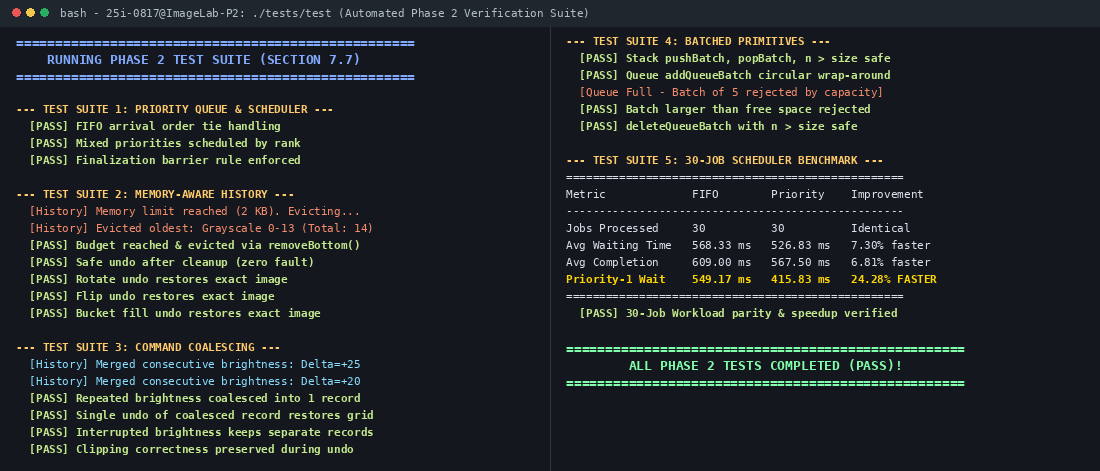
\includegraphics[width=0.96\textwidth,height=5.2cm,keepaspectratio]{p2_test_terminal_wide.png}\\[2pt]
    {\footnotesize \textbf{Figure 4:} Automated test runner terminal output confirming 100 percent test pass across all required suites.}
\end{center}

\vspace{0.2cm}
\begin{center}
    {\Large \textbf{Section 7: Known Limitations and Architectural Tradeoffs}}
\end{center}

\begin{itemize}[leftmargin=1.2em,noitemsep,topsep=2pt,parsep=1pt]
    \item \textbf{Oldest Record Eviction Shifting Overhead:} Because history is stored in a contiguous dynamic array, calling \texttt{removeBottom()} requires shifting $S$ elements left by one position in $\mathcal{O}(S)$ time. While efficient for moderate history depths, a circular deque buffer could achieve eviction in $\mathcal{O}(1)$ time.
    \item \textbf{Non Coalescing Geometric Operations:} While consecutive brightness adjustments coalesce seamlessly, opposite geometric operations such as 90 degree clockwise and counterclockwise rotations currently create separate history records instead of cancelling out.
    \item \textbf{Clipped Pixel Storage Scaling:} In extreme brightness shifts applied to highly textured images, thousands of pixels may clamp simultaneously at $0$ or $255$, which increases the memory footprint of the coordinate list stored in \texttt{clippedList}.
    \item \textbf{Bounded Pipeline Queue Capacity:} The job pipeline enforces a hard capacity limit of 100 jobs. Heavy batch workloads exceeding this ceiling are safely rejected and require manual drainage before new jobs can be scheduled.
\end{itemize}

\end{document}
